\documentclass[12pt]{article}
\usepackage{fullpage}
\usepackage{amsthm}
%\usepackage{amsmath}
\usepackage{mathtools}
\usepackage{amssymb}
\usepackage{todonotes}
\usepackage{tikz}
\usepackage{thmtools,thm-restate}
\usepackage{setspace}
\usepackage[colorlinks]{hyperref}
\usepackage{extramarks}
\usepackage{enumerate}
\usepackage[outline]{contour}
\usepackage{fancyhdr}
\usepackage{graphicx}
\graphicspath{ {./images/} }
% Font
\usepackage[rm,light]{roboto}
\usepackage[T1]{fontenc}
\begin{document}
\noindent
\begin{minipage}[t]{0.70\linewidth}
    \begin{flushleft}
        {\huge \textbf{CS253A}}\\
        \rule{0mm}{5mm}%
        {\large \textbf{\\Software Development And Operations}}\\
        \rule{0mm}{5mm}%
        {\normalsize \textbf{ Indian Institute of Technology, Kanpur}}\\
        \rule{0mm}{8mm}%
        {\large \textit{ \textbf{Anjali Rana \\ \rule{0mm}{5mm} Roll No. : 190147}}}    
    \end{flushleft}

\end{minipage}
\hfill
\begin{minipage}[t]{0.30\linewidth}
    \centering
    {\huge Assignment}\\ \rule{0mm}{18mm} \scalebox{5}{5}\\~\\
        Date of Submission:\\ March 27 2021

\end{minipage}

\rule{0mm}{0.5mm}%

{\centering \rule{0.99\linewidth}{1pt} }
\onehalfspacing
\thispagestyle{plain}
%\maketitle

\begin{center}
\rule{0mm}{40mm}%
    {\Huge \textbf{VIRAT KOHLI}}
\end{center}
\rule{0mm}{15mm}%
    Virat Kohli was born on 5 November 1988 in Delhi into a Punjabi Hindu family. His fatherworked as a criminal lawyer and his mother. According to his family, when he was three-years old, Kohli would pick up a cricket bat, start swinging it and ask his father to bowl at him.


    Virat Kohli is an Indian international cricketer and he is counted amongst the top sportsmen in India. He is considered to be among the best batsmen in the present era. He is known for his dependable and powerful batting style and has single-handedly won several matches for India. 

\newpage
    
    Kohli's debuts in different formats of matches is shown below:
    
    \textbf{Test Debut} : vs West Indies at Sabina Park, Jun 20, 2011
    
    \textbf{ODI debut} : vs Sri Lanka at Rangiri Dambulla International Stadium, Aug 18, 2008
    
    \textbf{T20 debut} :  vs Zimbabwe at Harare Sports Club, Jun 12, 2010
    
    \textbf{IPL debut} : vs Kolkata Knight Riders at M.Chinnaswamy Stadium, Apr 18, 2008\\
    
    Since the debuts, he has played many matches. The following graph shows the number matches of each category played by him till now. He has played maximum number of ODIs, followed by IPL and almost equal no. of Tests and T20I.

\begin{figure}[h]
\begin{center}
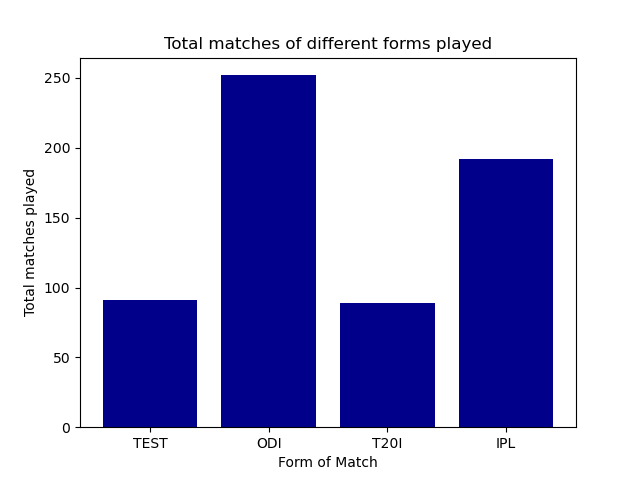
\includegraphics[width=1\linewidth]{assign/Bar.png}
\end{center}
\end{figure}
\newpage

\begin{figure}[h]
\begin{center}
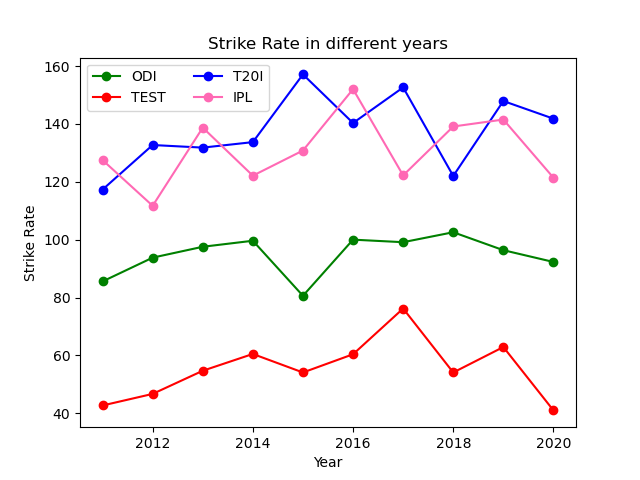
\includegraphics[width=1\linewidth]{assign/Group_line.png}
\end{center}
\end{figure}
     Kohli is considered to be among the best batsmen in the present era. It is really fascinating to look at his strike rate variations over years in different forms of cricket.\\ In ODI, his strike rate has been almost constant.\\ In tests, he has lowest strike rate among all formats of matches, since in tests, batsmen try not to lose wicket and thus play slowly.\\ In IPL and T20I, batsmen are expected to hit boundaries as much as they can, and it is evident from the graph that Kohli has maintained appreciably high strike rate in T20s, but it is very irregular.
\newpage

    
    
\begin{figure}
    \centering
    \subfloat{{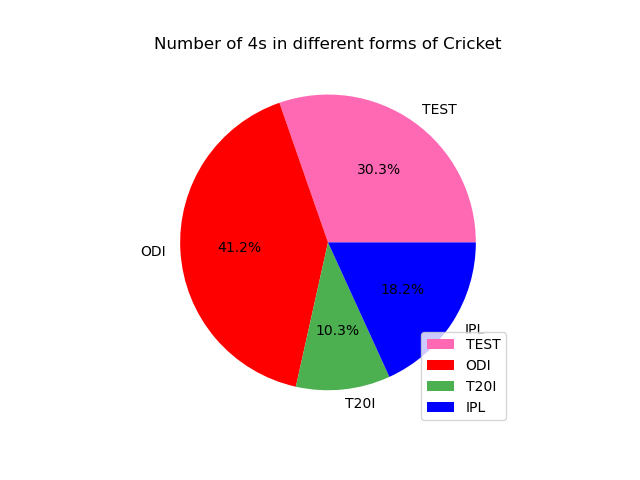
\includegraphics[width=10cm]{Pie_4s.png} }}
    \qquad
    \subfloat{{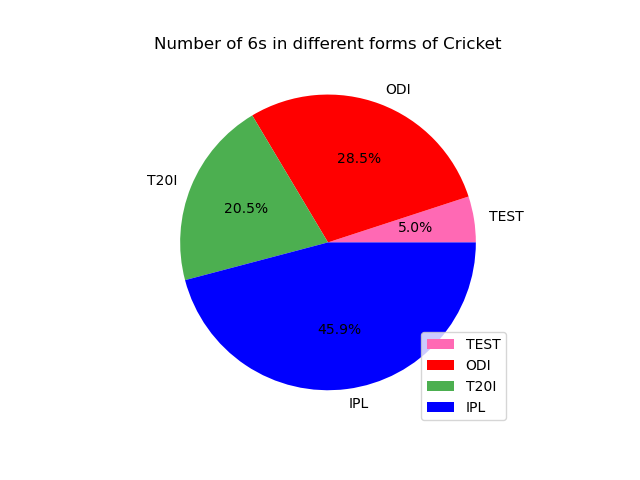
\includegraphics[width=10cm]{assign/Pie_6s.png} }}
    \label{fig:example}
\end{figure}

\rule{0mm}{18mm}
Now, if we try to compare boundaries hit by Kohli in different cricket formats, we get an expected result that in Tests, he had hit the lowest 6s while highest in IPLs. Interestingly, he has hit more 4s in ODIs and tests than in T20s. Almost $\frac{3}{4}^{th}$ of the 4s had been hit in ODIs and Tests. He had hit most 6s in IPL, almost half of all the 6s hit by him till now, followed by ODI
\newpage


    Kohli has scored very high scores in his career till now over years. Initially, his highest scores were on ODIs but in recent years, his highest scores come from Test crickets. This shows he has learned how to play maturely.
    
    
    \begin{figure}[h]
    \begin{center}
    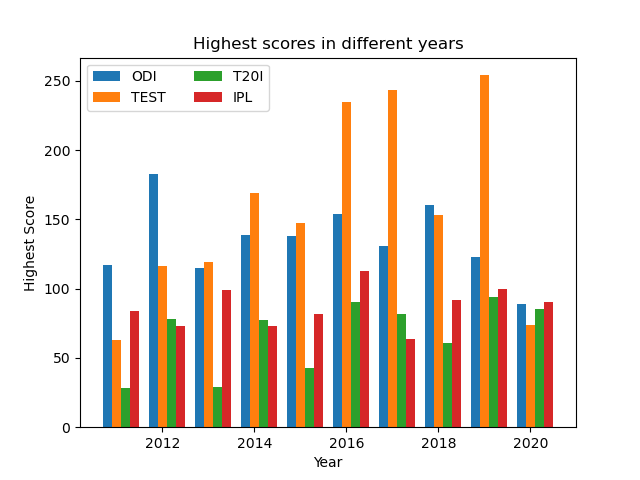
\includegraphics[width=1\linewidth]{assign/Group_bar.png}
    \end{center}
    \end{figure}
    
    
    \rule{0mm}{10mm}
    As per the above graph, clearly Kohli has scored at par wrt other categories in Tests. In 2019, he scored maximum score of his career in Test. If we make an approximate analysis, we can see that his average maximum score is around 150 in different categories, which is really appreciable and shows his efficient batting skills. Also, his highest scores in IPL is more than his highest score in T20I almost in every year. 
\newpage
    
     Kohli, along with playing safe in tests, is also a master at hitting boundaries. But, he has hit more 4s than 6s in his career. If we compare the two yearwise we get the follwing graph.
    \begin{figure}[h]
    \begin{center}
    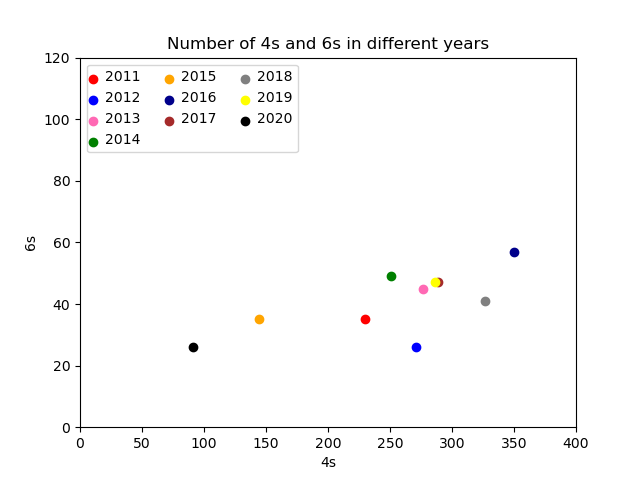
\includegraphics[width=1\linewidth]{assign/Scatter.png}
    \end{center}
    \end{figure}
    \rule{0mm}{20mm}
    Above is a detailed graph of yearwise boundaries and comparision between 4s and 6s hit by Kohli. It is evident from the graph that Kohli hits around 7 times the number of 4s as 6s in a year. (40 average 4s and 280 average 6s). Every year, almost equal number of boundaries are hit by him, in which 4s are at par with 6s.
\newpage



\newpage


 
\end{document}